%Adaped by Sumesh A K (ak_sumesh@cb.amrita.edu) 2026
% THESIS PART 2 of 2: Chapter 4 (Results and Inferences), Chapter 5 (Conclusion and Future Enhancements),
% References and Appendix. Part 1 holds the title page, front matter and Chapters 1-3.
% Compile this file as its own project/main document, then merge the PDFs: Part 1 (without its last
% reference page(s)) followed by Part 2.
%
% >>> SET THIS AFTER COMPILING PART 1: the page number of the first page of Chapter 4 =
% >>> (page number printed on the last page of Chapter 3 in Part 1) + 1.  (see the line \newcommand{\partTwoStartPage} below)
%\documentclass[PhD,two side]{ugthesis}
%\documentclass[MS]{ugthesis}
\documentclass[MTech]{ugthesis}
%\documentclass[BTech]{ugthesis}
\usepackage{times}
\usepackage{dashrule}
\usepackage{t1enc}
\usepackage{tikz}
\usepackage{subfigure}
\usepackage{setspace}
\usepackage{geometry}
\usepackage{graphicx}
\usepackage{epstopdf}
\usepackage{lscape}
\usepackage{fancyhdr}
\usepackage{natbib}
\usepackage{hyperref} % hyperlinks for references.
\usepackage{amsmath} % easier math formulae, align, subequations \ldots
\usepackage{amssymb}
\usepackage{wasysym}
\usepackage{titlesec}
\usepackage{textcomp}
\usepackage{pifont}
\usepackage[toc,page]{appendix}
\usetikzlibrary{decorations.pathmorphing}
\usetikzlibrary{shapes,arrows,shadows,patterns}
\usepackage[printonlyused]{acronym}
\setcounter{MaxMatrixCols}{20}
\captionsetup[figure]{labelfont=bf}
\newcommand{\RomanNumeralCaps}[1]
    {\MakeUppercase{\romannumeral #1}}
    \appendixpageoff
\renewcommand{\appendixpagename}{APPENDIX} % Changes the title page
\renewcommand{\appendixtocname}{APPENDIX}  % Changes name in TOC
\begin{document}

% >>> EDIT THIS NUMBER: first page number of Chapter 4 (= last page number of Chapter 3 in Part 1, plus 1)
\newcommand{\partTwoStartPage}{28}

% Continue the numbering of Part 1: Chapters 1-3 are in Part 1, so the first chapter here is Chapter 4.
\setcounter{chapter}{3}
\pagenumbering{arabic}
\setcounter{page}{\partTwoStartPage}
%------------------------------------------------------------------------------------------------%
\chapter{RESULTS AND INFERENCES}
\label{chap:results}

This chapter reports what has been measured so far: the behaviour of the prior, the posterior probabilities, the structural properties of the graphs, and the forecasting results at the five-minute horizon for one seed. The chapter states plainly which comparisons the current evidence can and cannot settle.

\section{Behaviour of the Prior}
Detrending is what gives the prior its contrast. On raw series, the median absolute correlation between candidate pairs is 0.84; practically every pair looks strongly related, and a prior built on such values would say nearly the same thing about every edge. After removing the time-of-day profile, the detrending step of Chapter 3, the median falls to 0.44, and the mapped prior $\eta$ spreads over $[0.05, 0.95]$ with mean 0.51. The prior is thus centred near neutrality, informative at the extremes, and incapable of forcing any edge in or out on its own.

\section{Posterior Probabilities}
All 2,056 units converged under each of the three priors, with at most seven units requiring the SLSQP retry. Table~\ref{tab:pstats} summarises the distribution of the pooled probabilities $P$ over candidate entries.

\begin{table}[htpb]
\small
\renewcommand{\arraystretch}{1.4}
\centering
\caption{Distribution of posterior inclusion probabilities over the 138,548 candidate entries, per prior.}
\label{tab:pstats}
\begin{tabular}{|p{4.2cm}|c|c|c|}
\hline
Share of entries & Flow prior & Uniform prior & Shuffled prior \\ \hline
$0.05 < P < 0.95$ & 45.3\% & 49.4\% & 47.3\% \\ \hline
$P > 0.99$ & 38.7\% & 38.2\% & 38.6\% \\ \hline
$P < 0.01$ & 0.4\% & 0.0\% & 0.3\% \\ \hline
$P \ge 0.5$ & 63.5\% & 64.3\% & 65.7\% \\ \hline
\end{tabular}
\end{table}

Two readings follow. First, the probabilities are informative rather than saturated: under every prior, close to half of the entries lie strictly between 0.05 and 0.95, so the model is genuinely grading edges instead of making binary decisions. Second, the three distributions are similar in aggregate; the prior shifts individual pairs (in a sixty-unit pre-training check, 14.3\% of entries moved by more than 0.10 when the flow prior replaced the uniform one) but does not reshape the overall distribution. The data, through the residual covariance, dominate the prior, which is how a prior is supposed to behave when the sample is large.

\section{Properties of the Graphs}
Table~\ref{tab:graphs} lists the edge counts of the final graphs and their pairwise agreement, measured by the Jaccard index of the edge sets.

\begin{table}[htpb]
\small
\renewcommand{\arraystretch}{1.4}
\centering
\caption{Graph sizes and edge-set agreement (Jaccard index) by horizon.}
\label{tab:graphs}
\begin{tabular}{|p{5.6cm}|c|c|c|c|}
\hline
 & $h=1$ & $h=3$ & $h=6$ & $h=12$ \\ \hline
Edges, PEM variants (each) & 40{,}794 & 49{,}874 & 49{,}936 & 49{,}936 \\ \hline
Edges, VAR-only & 40{,}794 & 50{,}401 & 50{,}692 & 50{,}694 \\ \hline
Flow vs.\ uniform & 0.975 & -- & 0.932 & -- \\ \hline
Flow vs.\ shuffled & 0.960 & -- & 0.897 & -- \\ \hline
Flow vs.\ VAR-only & 0.907 & 0.761 & 0.728 & 0.672 \\ \hline
\end{tabular}
\end{table}

The pattern anticipates the forecasting results. The three prior variants select almost the same edges, agreeing on 96--98\% at five minutes and still above 90\% at thirty minutes; whatever the prior contributes must therefore act through edge \emph{weights} more than through edge selection, and differences between these variants should be expected to be small. The PEM-weighted graph and the VAR-only graph, by contrast, diverge substantially as the horizon grows, down to 0.67 agreement at one hour; the comparison between the proposed graph and the VAR-only ablation is consequently the one with room to show an effect, and it is the comparison on which the usefulness of PEM has been staked.

\section{Forecasting Results at the Five-Minute Horizon}
Table~\ref{tab:res5} reports the test metrics of the three PEM-based graphs, trained and evaluated under the protocol of Chapter 3 with seed 42, together with the reference models trained earlier under identical settings. Each model was trained for 20 epochs in about 5.4 GPU-hours, and the test set was touched once per run.

\begin{table}[htpb]
\small
\renewcommand{\arraystretch}{1.4}
\centering
\caption{Test results at the five-minute horizon ($h=1$), seed 42, in vehicles per 5 minutes. Masked MAPE uses targets of at least 10 vehicles.}
\label{tab:res5}
\begin{tabular}{|p{5.2cm}|c|c|c|c|}
\hline
Model & RMSE & MAE & Masked MAPE (\%) & $R^2$ \\ \hline
Historical average & 54.92 & 33.24 & -- & -- \\ \hline
Road graph & 29.76 & 19.34 & 11.89 & -- \\ \hline
VAR-weighted road graph & 28.10 & 18.36 & 10.49 & -- \\ \hline
Graph-free (identity) & 27.58 & 16.87 & 11.19 & -- \\ \hline
Proposed (flow prior) & 27.30 & 17.95 & 11.21 & 0.9715 \\ \hline
Uniform prior & 25.88 & 16.48 & 10.02 & 0.9743 \\ \hline
Shuffled prior & 25.86 & 16.55 & 10.39 & 0.9744 \\ \hline
\end{tabular}
\end{table}

\begin{figure}[htpb]
\centering
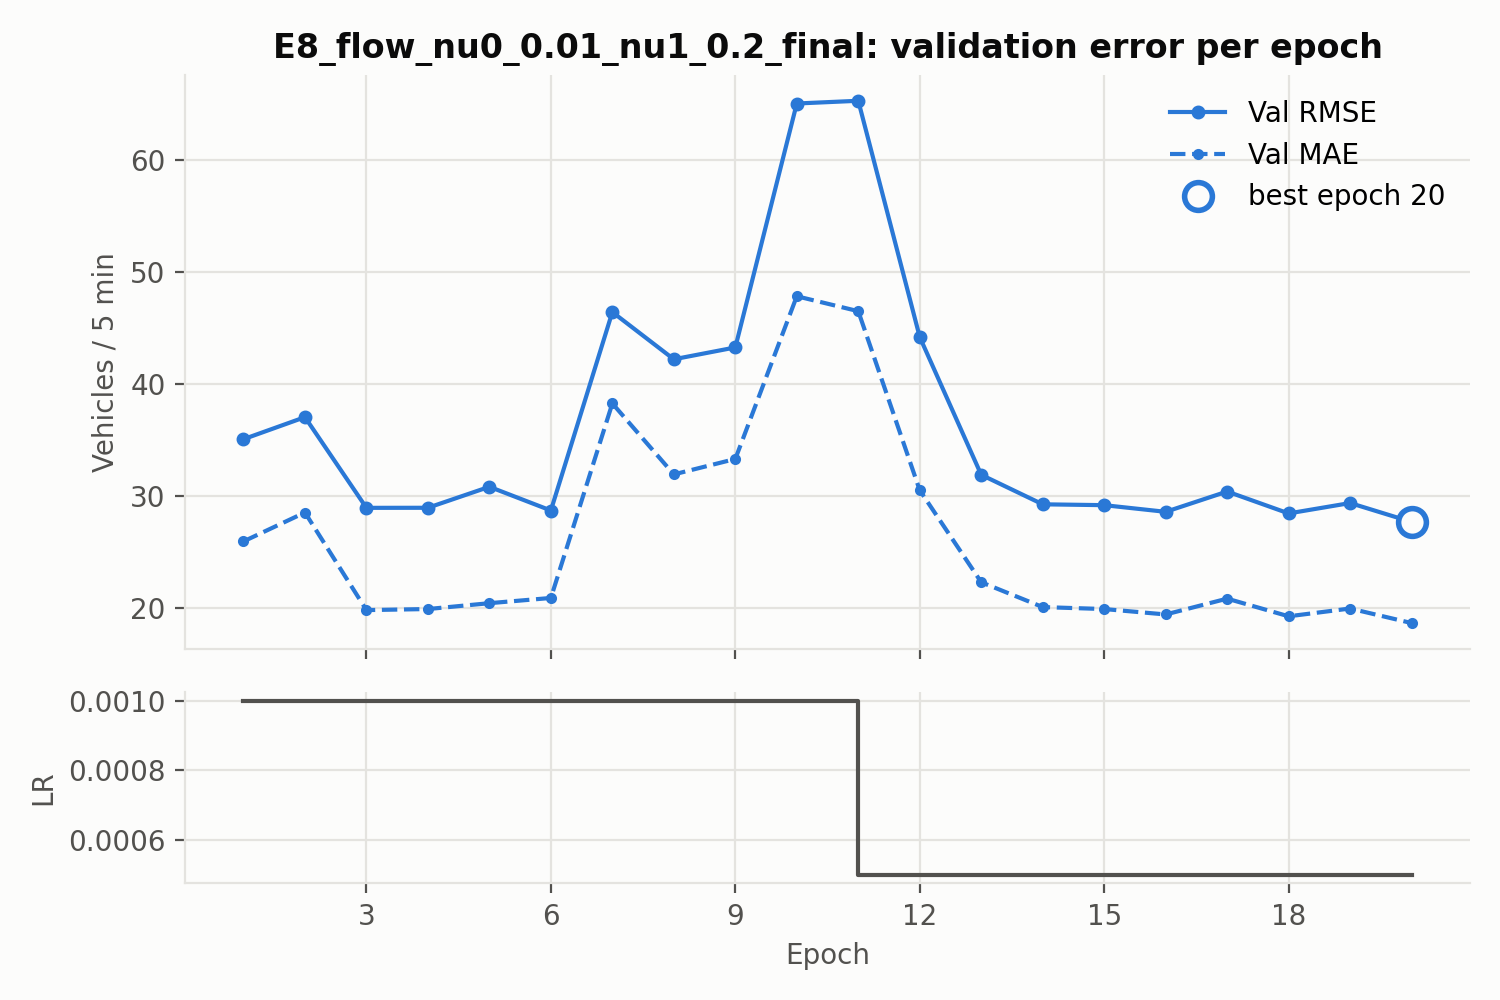
\includegraphics[width=0.85\textwidth]{fig_training_curve_flow.png}
\caption{Validation error per epoch for the proposed (flow-prior) run at $h=1$, seed 42. The disturbance around epochs 7--12 and the late best epoch are discussed in Section~\ref{sec:stability}.}
\label{fig:curve}
\end{figure}

\section{Inferences}
\label{sec:infer}

The honest reading of Table~\ref{tab:res5} has three parts.

\textbf{The PEM-based graphs are competitive.} All three beat the road graph by 2.5 to 3.9 RMSE and also lie below the VAR-weighted road graph and the graph-free model on this seed. This is encouraging but, on one seed, not yet a claim: reference runs repeated with a second seed have shown shifts of up to 1.4 RMSE from the seed alone (the VAR-weighted road graph moved from 28.10 to 26.71, and the road graph from 29.76 to 30.13), so single-seed margins of this size cannot be ruled out as random. The repetition seeds are specified and the runs are queued.

\textbf{The informed prior has not shown a benefit.} The proposed flow prior reached 27.30 while its two controls reached 25.88 and 25.86. The controls' near-identical scores say that the prior's information content made no measurable difference to the forecast, and the proposed variant's higher error is itself within the seed spread and may not be a real deficit. Neither direction of the prior question is settled, but the burden of proof now lies on the prior: at the five-minute horizon, where the three graphs share up to 97.5\% of their edges, there was little room for it to act, and it did not.

\textbf{The decisive comparison is still open.} The VAR-only ablation, the variant that determines whether PEM contributes anything at all, has been built and verified but its training run was not complete at the time of writing. Until it is scored across seeds, no statement about the value of the probability model is made. Likewise, the fact that the two controls (25.9) outperformed every external reference on this seed suggests that the combination of VAR impulse responses with PEM weighting may be the active ingredient rather than the prior, but this, too, is a hypothesis for the pending runs, not a finding.

\section{Training Stability}
\label{sec:stability}
All runs at this scale show a degree of optimisation noise, and it should be recorded rather than smoothed over. The flow-prior run suffered a loss spike around epoch 10, with validation RMSE briefly rising from about 29 to 65 before recovering (Figure~\ref{fig:curve}); the uniform and shuffled runs showed smaller disturbances of the same kind, and in all three the best epoch arrived late (epochs 17--20), with validation error still trending downward at the end of the 20-epoch budget. Two consequences follow. The fixed 20-epoch budget may truncate training before convergence, identically for every variant, which is fair between variants but inflates the influence of where each run happens to stop; and the spikes add variance to single-run comparisons, reinforcing the multi-seed requirement already built into the protocol. Whether the spikes relate to the near-unit eigenvalue of the fitted VAR or are ordinary learning-rate effects has not been established.

\begin{figure}[htpb]
\centering
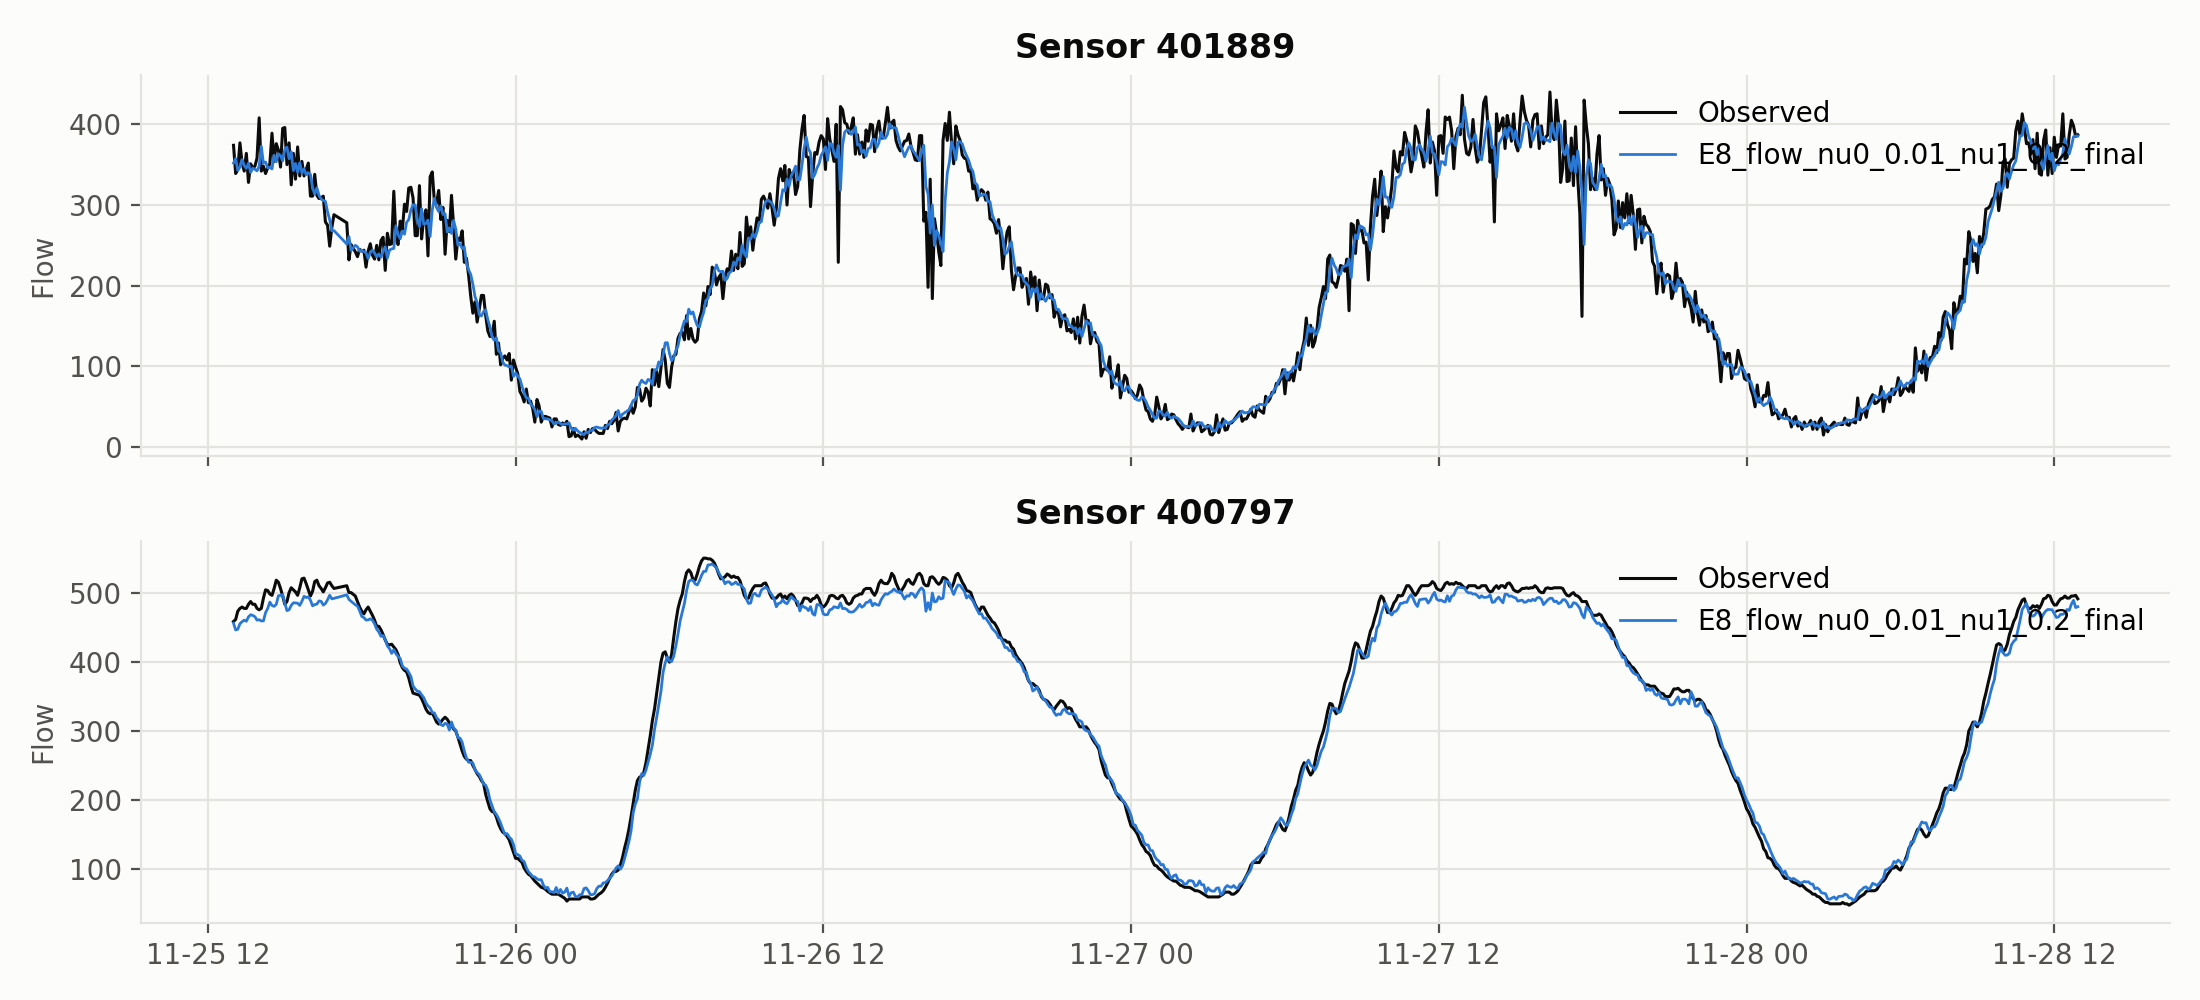
\includegraphics[width=0.95\textwidth]{fig_example_series_flow.png}
\caption{Observed and predicted flow for a median-flow and a high-flow sensor over the first three test days, proposed (flow-prior) model at $h=1$. The model tracks the daily structure closely at this horizon.}
\label{fig:series}
\end{figure}

%------------------------------------------------------------------------------------------------%
\chapter{CONCLUSION AND FUTURE ENHANCEMENTS}

\section{Conclusion}
This thesis set out to replace the road graph of a fixed traffic forecaster with a graph estimated from the traffic itself, built so that each of its ingredients can be tested in isolation. The construction combines directed, horizon-specific effects from a topology-aware vector autoregression with posterior edge probabilities from a spike-and-slab precision model, informed by a prior computed from the correlation of detrended training flow. The design contributes safeguards that are easy to state and were enforced mechanically: every estimator sees training rows only, the forecaster is never modified, graph artefacts carry their own provenance and are verified against the run that uses them, and the method ships with the controls needed to falsify it, a uniform prior, a shuffled prior, and a PEM-free ablation.

The evidence available at this stage supports a measured summary. The construction behaves as designed: the detrended correlation prior is informative without being dogmatic, the posterior probabilities grade edges rather than saturating, and the resulting graphs are structurally sound at every horizon. In the first forecasting comparison, at the five-minute horizon on one seed, all three PEM-based graphs outperformed the road graph, and the two control priors produced the best scores of any model evaluated; however, the informed prior did not beat its controls, and the margins involved are comparable to the variation induced by the random seed. The comparisons that will decide the two central questions, whether PEM improves on the VAR-only graph and whether any variant's advantage survives across seeds and horizons, are specified, queued, and deliberately left unprejudged.

\section{Limitations}
\begin{itemize}
\item Forecasting evidence currently covers one horizon and one seed; all conclusions drawn from it are provisional by construction.
\item The VAR-only ablation, the decisive control for the probability model, has not yet been scored.
\item The prior is undirected and partly reflects spatial proximity, since candidate pairs are defined through road units.
\item The fitted VAR is marginally non-stationary (largest companion eigenvalue 1.05), which complicates the interpretation of impulse-response magnitudes across horizons.
\item Training shows loss spikes and late best epochs within the fixed 20-epoch budget, adding noise to single-run comparisons.
\item The study uses one region and one year of data, and GPU training is not bit-reproducible, so exact numbers are reproducible only in distribution.
\item The PEM scale parameters were revised once, before any training, on the basis of a pre-training probability check; the revision is reported in Chapter 3.
\end{itemize}

\section{Future Enhancements}
The immediate programme is completion of the designed evaluation: the VAR-only ablation at all horizons, seeds 7 and 123 for every variant, and the 15-, 30- and 60-minute horizons, where the graphs differ most and a horizon-conditioned construction has the most room to justify itself. Significance testing on per-sensor errors and forecast-difference tests will accompany the multi-seed results. Beyond the designed evaluation, three extensions follow naturally. External baselines, including a recurrent model without any graph and an established graph-based forecaster such as Graph WaveNet \citep{wu2019graphwavenet}, would place the framework among published methods rather than only among its own ablations. The training instability deserves a diagnosis, since a stabler optimisation would sharpen every comparison in the study. Finally, if the correlation prior continues to show no effect, the prior mapping itself (the affine map of Chapter 3) can be made more aggressive, for example by percentile scaling, turning the present negative indication into a usable design conclusion about how much prior information a well-sampled precision model can absorb.

%------------------------------------------------------------------------------------------------%

%%%%%%%%%%%%%%%%%%%%%%%%%%%%%%%%%%%%%%%%%%%%%%%%%%%%%%%%%%%%
% Bibliography (complete list: all references of the thesis, including those cited only in Part 1).
\nocite{*}
\begin{singlespace}
  \bibliography{thesis_refer} %Enter your .bib file name here
\end{singlespace}
\addcontentsline{toc}{chapter}{REFERENCES}
\appendix

\begin{appendices}
\chapter*{APPENDIX}
\section*{A. Graph artefact format}
Each graph is stored as a compressed archive holding the adjacency matrix (rows as targets, columns as sources), the ordered sensor list, the training-split boundary, the forecast horizon, the top-$K$ setting, and the identifier of the producing run. The training harness refuses any artefact whose sensor list, split boundary, orientation or horizon disagrees with the run configuration, so a mismatched graph cannot silently enter a result.

\section*{B. Build-time checks}
Every graph build re-verifies: $\Psi_1 = A_1$ (orientation and recursion), symmetry of $P$, zero diagonals, the in-degree bound $K$, that each retained edge lies in the support of $P$, that the PEM-weighted scores never exceed the unweighted scores, and that no LiNGAM module is imported and no contemporaneous-structure file is opened anywhere in the build. A build aborts if any check fails.
\end{appendices}
%%%%%%%%%%%%%%%%%%%%%%%%%%%%%%%%%%%%%%%%%%%%%%%%%%%%%%%%%%%%
  \end{document}
